\chapter{Evaluation}
\section{Evaluation on Datasets}
\label{sec:EvaluationOnDatasets} % Now, we can use "\autoref{sec:<my-label>}" to refer to this chapter
The face segmentation network was tested on two different datasets 1.) The Caltech occluded faces in the wild (COFW) and 2.) parts-labeled LFW Dataset of the University of Massachusetts \cite{LFW_dataset}. Both datasets are designed to present faces in real-world conditions. The COFW dataset provides 29 landmarks and a bounding box for all 507 images. The original LFW dataset contains 13'000 images of 1'680 different subjects. Each face is labeled with the name of the subject. This database is actually meant to test facial recognition/verification algorithms on it. Nevertheless, we tested the segmentation of the FCN on the 500 image parts-LFW validation set. For each image there is a ground truth segmentation, which makes it possible to measure the quality of the FCN in numbers.
\\

\subsection{COFW}
Since on the COFW dataset, only landmarks and bounding-boxes are given, the segmentation had to be evaluated qualitatively. We weren't able to count the correctly labeled pixels of the FCN with respect to a ground-truth mask. To increase the precision of the network, we cropped the images according to the given bounding-boxes. Because the bounding-boxes were only inluding the eyes and the mouth of the subject, we had to add an offset which was determined by eye. Nevertheless, we tried to reconstruct the graphic on Nirkis \cite{nirkin2018_faceswap} github-repository 'face\_segmentation'.
\begin{figure}[h]
	\centering
	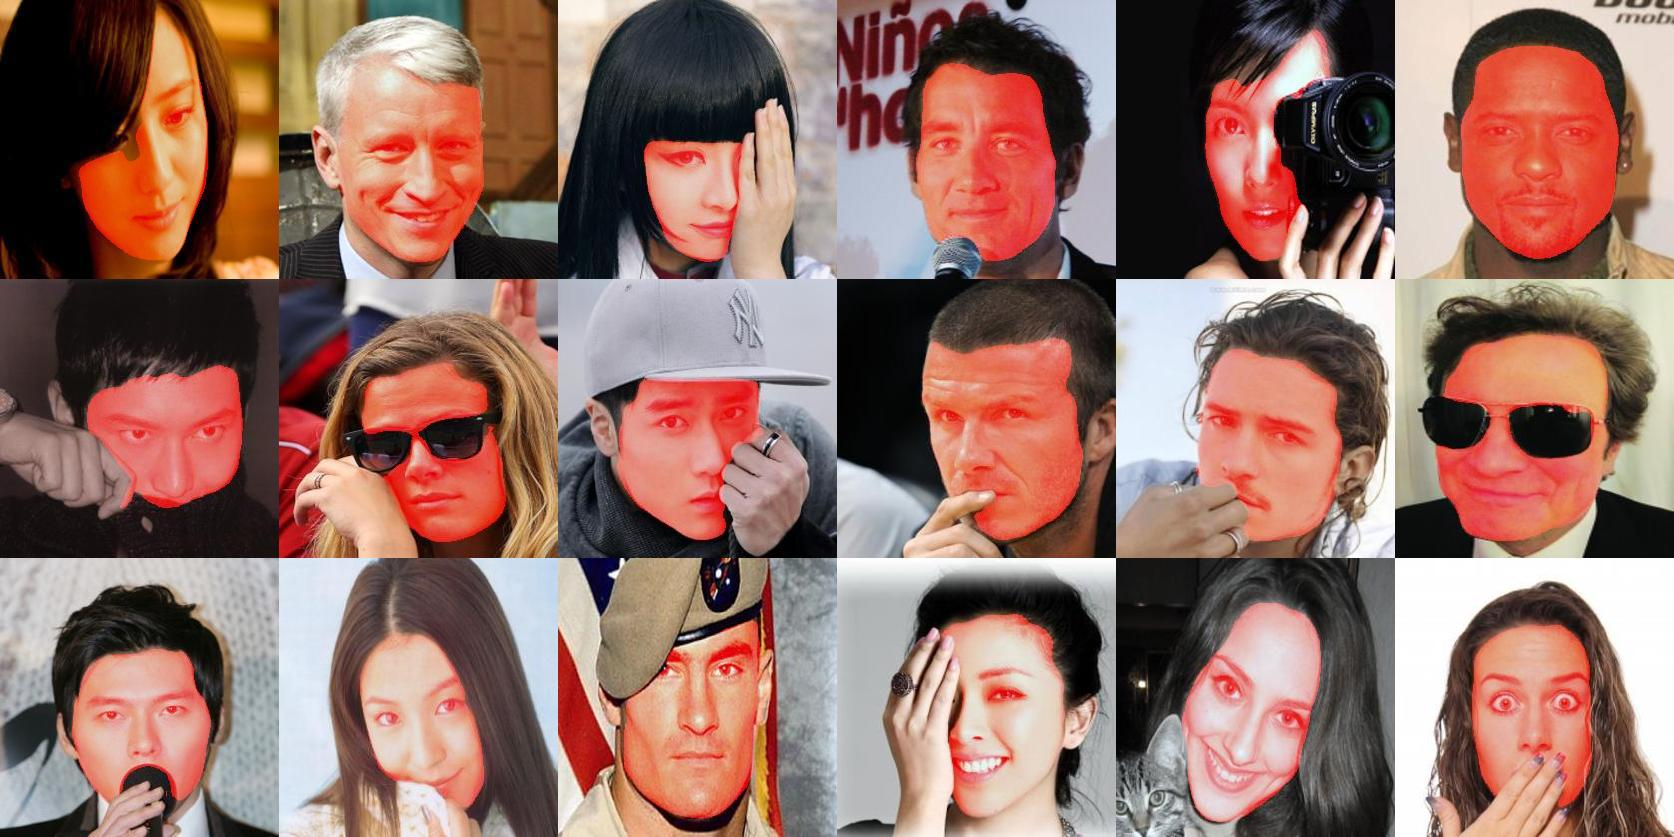
\includegraphics[width=1\textwidth]{Figures/myMatrix.jpg}
	\caption{18 images of the COFW Dataset overlayd with the FCN output (in red). The given box was extended upwards by 80\%, to the right and left it was 55\% and downwards t was 5\%.}
	\label{figure2}
\end{figure}


\begin{figure}
	\centering
	\subbottom[An facial-image with the segmentation of the FCN highlited in red]{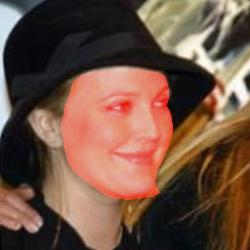
\includegraphics[width=0.4\textwidth]{Figures/chap2/drew/drew_original.jpg}\label{fig:drew:sf1}}
	\subbottom[The provided ground-truth segmentation of the image \ref{fig:drew:sf1} overlaid with the mask of the FCN (red)]{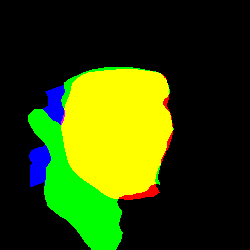
\includegraphics[width=0.4\textwidth]{Figures/chap2/drew/drew_segments.png}\label{fig:drew:sf2}}
	
	
	\subbottom[An facial-image with the segmentation of the FCN highlited in red]{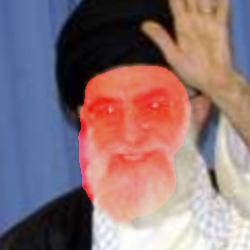
\includegraphics[width=0.4\textwidth]{Figures/chap2/ali/ali_original.jpg}\label{fig:ali:sf3}}
	\subbottom[The provided ground-truth segmentation of the image \ref{fig:ali:sf3} overlaid with the mask of the FCN (red)]{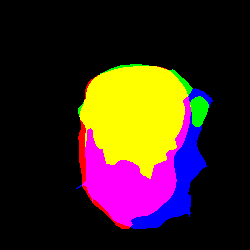
\includegraphics[width=0.4\textwidth]{Figures/chap2/ali/ali_segments.png}\label{fig:ali:sf4}}
	\caption{Plots of four Turing machines}
	\label{fig:tm}
\end{figure}

\subsection{Parts-LFW}
In the Parts-LFW dataset, we had a ground-truth mask for every image. The mask distinguishes between hair, skin and background. We iterated trough all the provided groud-truth masks and overlaid them with the segmentation of the FCN. The evaluation is quite impressive. The FCN performs very good in segmenting only pixels which belong to the face. In average over the 500 images of the Parts LFW dataset, there are $98.5\%$ right non-segmentations (only 1.5\% background in the segmentation). On the other hand, only $85.4\%$ of all the pixels which belong to the face are segmented as face pixels wich isn't a good but accepable result. Figures \ref{fig:drew:sf1} and \ref{fig:drew:sf2} depict such a face image and it's mask. Unfortunately, on the given mask, no distinction is made between face and other parts of the body, but everything is segmented as skin (Subfigures \ref{fig:drew:sf1} and \ref{fig:drew:sf2}). However, the bigger problem is that some faces have beards. The FCN of \cite{nirkin2018_faceswap} segmented facial hair which was excluded on the provided labels. So we had to manually remove these images (Subfigures \ref{fig:ali:sf3} and \ref{fig:ali:sf4}). To reduce the effort, we took the Parts-LFT Validation set containing 500 images. After removing the ones with a beard or mustache, we were left with 447 images. The results are summarized in Figure \ref{fig:Parts-LFW}\\
\\
%\vspace{.5cm}\\
\begin{figure}
\begin{center}
\begin{tabular}{l|l} \hline
	false-positives (hair) & 7.04\%\\ \hline
	false-positives (background) & 0.68\%\\ \hline
	right-segmentations & 85.87\%\\ \hline
	right non-sementations & 99.32\% \\ \hline
\end{tabular}
\end{center}
\caption{The averages over the 447 images of the PArts-LFW evaluation set of \cite{LFW_dataset}. The FCN recognizes (almost) only pixels, which also belong to the face (little false positives). By reducing from 500 to 447 images, we were able to reduce them. Unfortunately, there are many false negatives (skin pixels labeled as background).} 
\label{fig:Parts-LFW}
\end{figure}
%\vspace{.5cm}

\section{Evaluation on synthetic-data}
In order to evaluate the FCN on synthetic-data, we used the Parametric-Face-Image-Generator of \cite{parametric} to produce images of a random face in a given pose (see Figure \ref{fig:syntheticData_samples}). We extended the software so that it now renders occlusions over the face. Further, we changed the Parametric-Face-Image-Generator so it now generates a Ground-Truth-Mask, which classifies every pixel either as part of the face or as non-face.\\
\\
Nirkin et al. \cite{nirkin2018_faceswap} claim that both the face itself an the context of the face play an important role for the outcome of the segmentation. To measure this effect and reduce the impact of outliers, we repeat each experiment multiple times with a different face and a different backgroundimage. All images we use for the following tests were generated with the same illumination. Within a dataset The face stays the same within a whole set of images. Each experiment was repeated with multiple sets. For the results we use the average of all results.

\begin{figure}[h]
	\centering
	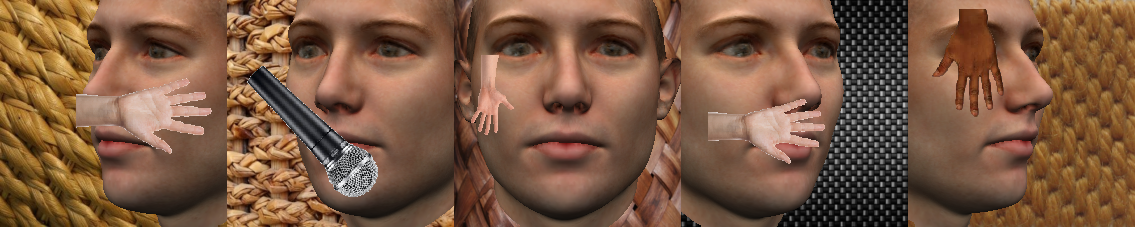
\includegraphics[width=\textwidth]{Figures/chap2/syntheticData_samples.png}
	\label{fig:syntheticData_samples}
	\caption{Five examples of the synthetic face images. The same face is shown with yaw angles $-45$\textdegree, $-25$\textdegree, $0$\textdegree, $25$\textdegree, and $45$\textdegree. The occlusion is randomly choosen and in a random orientation and position.}
\end{figure}

\subsection{Dpendence of the Euler angles}
Because we can now create synthetic face images in any desired pose, we first wanted to find out the accuracy of segmenting the FCN for the angles: Yaw, Roll, and Pitch. In order to do that, we produced with the tool of \cite{parametric} 101 face images for every angle from $-50$\textdegree to $50$\textdegree. In every picture, the face is turned one degree further. We evaluated each angle itself and every possible combination of the angles in order to create a hierarchy under the angles. We evaluated each angle itself and every possible combination of the angles (results in Figure \ref{fig:evaluation_angles})\\
\\
From the graphs of Figure \ref{fig:evaluation_angles} we can conclude that the roll angle is the most relevant for the FCN. The pitch-angle is less important and that the accuracy of the FCN is still good even with hith angles (least important). 

\begin{figure}[h]
	\centering
	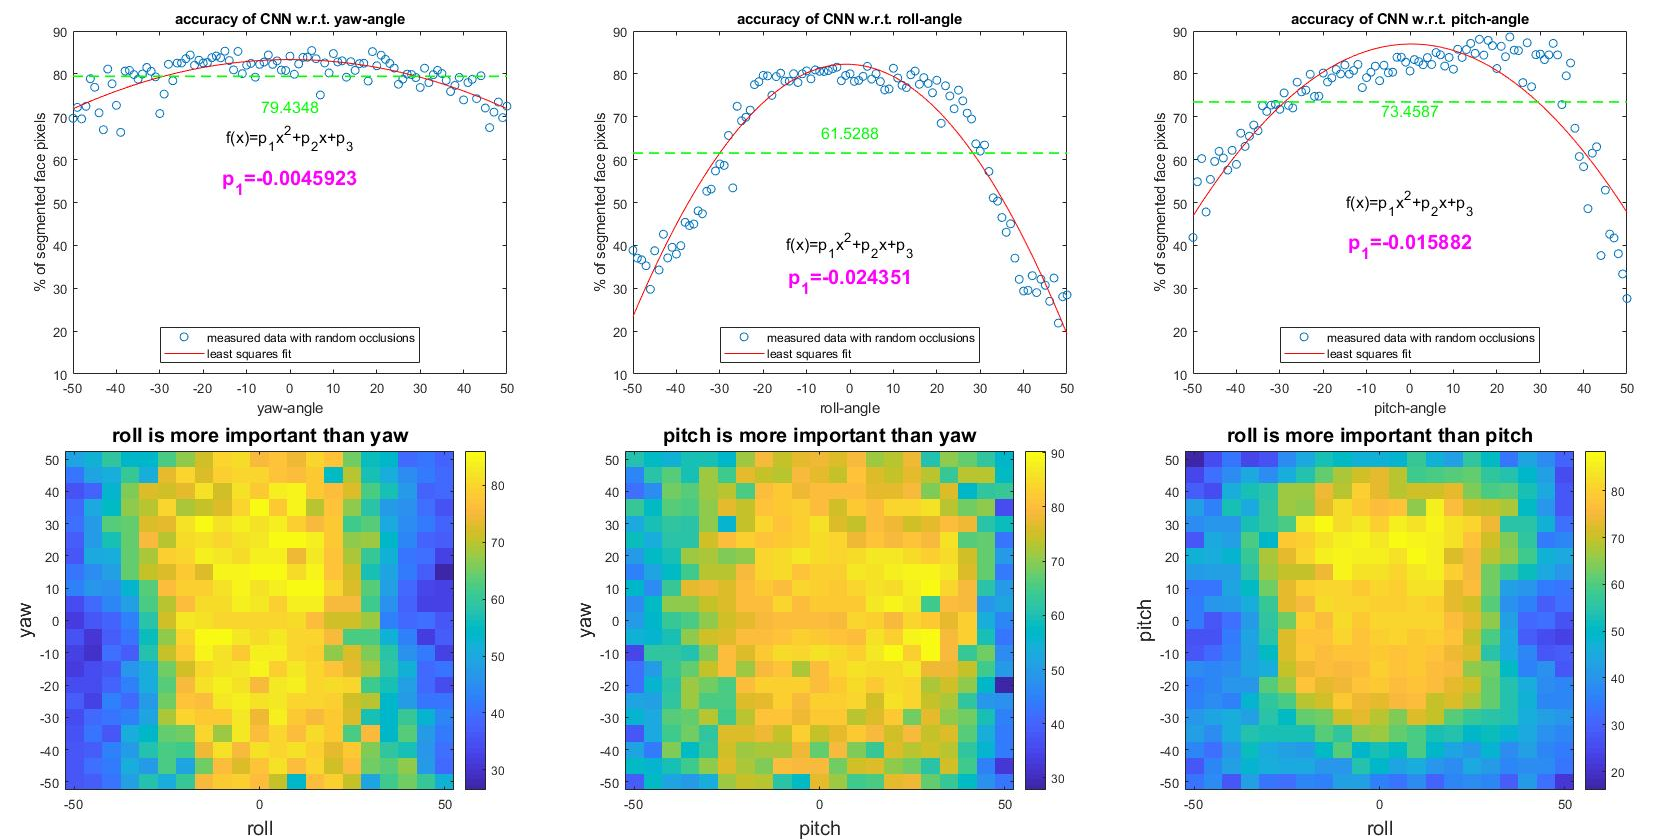
\includegraphics[width=\textwidth]{Figures/evaluation_angles.png}
	\caption{In the plots on the top row we see the segmetation accuracy in percent (on the y-axis) for every single image (with face angle from $-50$\textdegree to $50$\textdegree on the x-axis). The point cloud is approximated by a quadratic function via a least squares fit (red curve / $f(x)$). The first parameter of this function determines the opening angle ($p_1$). In the bottom row the colors indicate the segmentation accuracy. The brighter the color, the better the segmentation. In every plot, there is a cluster of high accuracy segmentations centered in the origin. The angle on whose axis the cluster has the lesser extent is the more important of the two. We call an angle important, when a small change of this angle leads to a failure of the FCN. }
	\label{fig:evaluation_angles}
\end{figure}

\subsection{random boxes as occlusions}
With the parametric-face-image-generator of \cite{parametric}, we produced about 5.2 thousand images of Which for every angle from $-40$\textdegree to $40$\textdegree  include 100 images of 5 different faces with 20 different occlusion levels. In the given table (Figure \ref{fig:angle_table}) all provided images show a face, from which 20\% of the pixels are occluded by a randomly colored box. We can optically verify, that 1) the yaw angle, despite the occluding box, hasn't much of an effect. 2.) In both situations, -40 and 40, of the roll angle, the result is not satisfying. 3.) In the third column, the segmentation with a negative pitch angle is much worse than with a positive one! Note that the results for each grid cell in figure \ref{fig:occVal40} is based on 5 segmentations (5200 images over all)!\\

% The source for this table was this post: https://stackoverflow.com/questions/2771856/centering-text-horizontally-and-vertically-in-latex
% To add padding for the cell contents: https://tex.stackexchange.com/questions/31672/column-and-row-padding-in-tables
\begin{figure}[h]
	\begin{center}
		\newcolumntype{C}{>{\centering\arraybackslash} m{2cm} }  %# New column type
		\begin{tabular}{m{1cm}|SC|SC|SC}
			& yaw & roll & pitch\\ \hline
			-40 & \subfloat{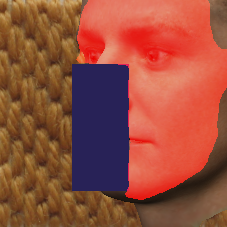
\includegraphics[width=0.1\textwidth]{Figures/-40_0_0_occVal_20.png}} &
			\subfloat{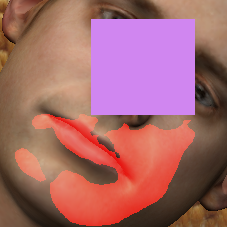
\includegraphics[width=0.1\textwidth]{Figures/0_0_-40_occVal_20.png}} &
			\subfloat{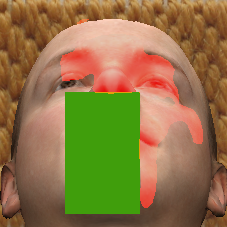
\includegraphics[width=0.1\textwidth]{Figures/0_-40_0_occVal_20.png}} \\ \hline
			40 & \subfloat{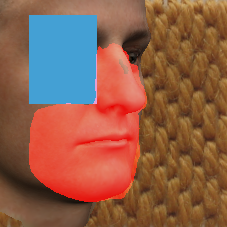
\includegraphics[width=0.1\textwidth]{Figures/40_0_0_occVal_20.png}} &
			\subfloat{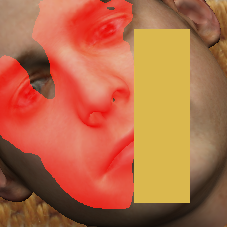
\includegraphics[width=0.1\textwidth]{Figures/0_0_40_occVal_20.png}} &
			\subfloat{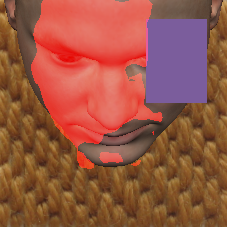
\includegraphics[width=0.1\textwidth]{Figures/0_40_0_occVal_20.png}} \\
		\end{tabular}
	\end{center}
	\caption{Based on these images, we can see that the roll angle (rotation) is the most sensitive, followed by the pitch angle (tilt), where the segmentation works better on positive angles than on negative ones. The most stable detection is at the yaw angle. It has the least influence on the segmentation.}
	\label{fig:angle_table}
\end{figure}
Although boxes as occlusions are very simpley and we're in control of the rectangle's size, we can occlude a given amount of the face region with this method, but in practice, exact rectangles are very rare. That's why we left it with the rectangles and used real-world objects (e.g. hands, microphones or sunglasses) as synthetic occlusions. Unlike Nirkin[1], we didn't use the landmarks of the face for this task. We placed them randomly on the image instead. Thats the reason why we use a second plot to show the percentage of occluded face pixels in the following.

\begin{figure}[h]
	\centering
	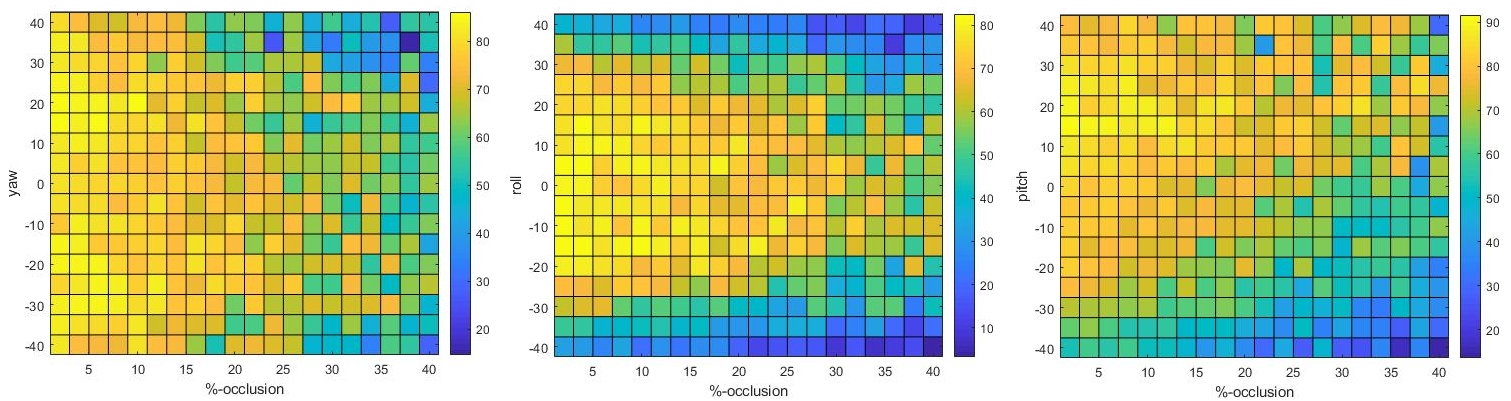
\includegraphics[width=\textwidth]{Figures/occVal_angles.png}
	\caption{The color of each grid cell indicates the accuracy of the segmentation of the FCN on a set of faces turned by the corresponding angle and occluded with a square, so that the corresponding amount of the face is masked. The brighter the color, the better the segmentation. On each plot, we would expect to see a triangle pointing to the right. This means that the combination of a large angle and a large occlusion make the face even more unsegmentable.}
	\label{fig:occVal40}
\end{figure}
We see that the segmentation is very sensitive to roll-angles and the FCN is not trained to segment faces in every rotation! Surprisingly, the yaw angle plays a subordinate role here. The right most plot tells us, that the sign of the pitch angle plays a significant role! Since we aren't able to determine at which angles exactly the FCN begins to fail,we repeated the experiment with a higher angle range:\\

\begin{figure}[h!]
	\centering
	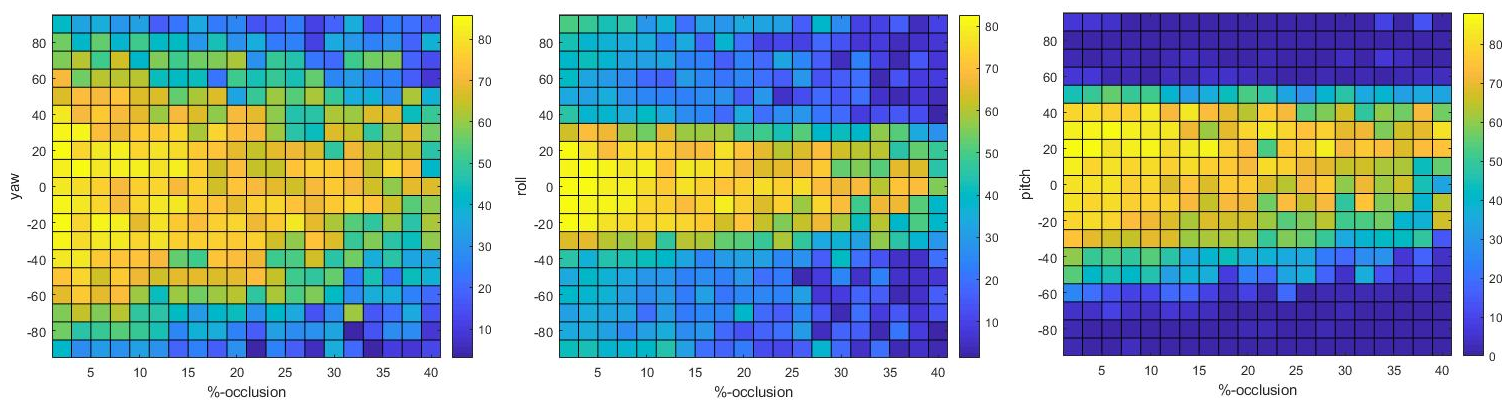
\includegraphics[width=\textwidth]{Figures/occVal_angles_90.png}
	\caption{This plot shows the outcome of a similar expreiment as snown in Figure \ref{fig:occVal40} with less resolution. All the angles (yaw, pitch and roll) range from $-90$\textdegree to $90$ \textdegree. The scale on the "\%-occlusion" stays the same as in Figure \ref{fig:occVal40} We can clearly see the limits of the FCN even with a occlusion of 2\%! Very interestig is the hard transition from good segmentations to bad segmentations in the two right plots.}
	\label{fig:occVal90}
\end{figure}

\section{Parametric-Face-Image-Generator}
As metioned at the beginning of this chapter, we extended the Parametric-Face-Image-Generator of \cite{parametric}. In our version the option "occlusionMode" in the configuration files can now be set to:
\begin{itemize}
	\item \textbf{"random"}: A randomly choosen occlusion image hides the picture in a random place.
	\item \textbf{"box"}: Boxes, filled with either an arbitrary color or gaussian-white-noise hide the image.
	\item \textbf{"box-whitenoise"}: Boxes, filled with gaussian-white-noise only.
	\item \textbf{"eyes"}: Black boxes hiding the eyes on the face in the image.
\end{itemize}
In addition to the output Images, the parametric-face-image-generator now provides masks as well. They can be used as ground truth for the position of the face and te occlusion.
